\chapter{Grundlagen}
\label{chap:basics}

\section{Statische Typsysteme für JavaScript}

Es gibt noch viele weitere: https://github.com/jashkenas/coffeescript/wiki/List-of-languages-that-compile-to-JS

\subsection{Flow}
  Flow beschreiben (und zwar mit entsprechender Fachsprache)

\subsubsection{Basistypen}

\begin{table}[tbp]
  \footnotesize
  \begin{tabularx}{\textwidth}{@{}ll@{}}
    \midrule
    \textbf{Basistyp}         & \textbf{Beispiel}                        \\
    \midrule
    Array type                 & \texttt{Array<{}number>{}}               \\
    Boolean literal type       & \texttt{true}                            \\
    Boolean type               & \texttt{boolean}                         \\
    Empty type                 & \texttt{empty}                           \\
    Exact object type          & \texttt{\{| prop: any |\}}               \\
    Function type              & \texttt{(string, \{\}) => number}        \\
    Generic type annotation    & \texttt{let v: <{}FlowType>{}}           \\
    Generics                   & \texttt{type Generic<{}T: Super> = T}    \\
    Interface type             & \texttt{interface \{ +prop: number \}}   \\
    Intersection type          & \texttt{type Intersection = T1 \& T2}    \\
    Mixed type                 & \texttt{mixed}                           \\
    Null literal type          & \texttt{null}                            \\
    Nullable type (Maybe type) & \texttt{?number}                         \\
    Number literal type        & \texttt{42}                              \\
    Number type                & \texttt{number}                          \\
    Object type                & \texttt{\{ {[}string{]}: number \}}      \\
    Opaque type                & \texttt{opaque type Opaque = number}     \\
    String literal type        & \texttt{'literal'}                       \\
    String type                & \texttt{string}                          \\
    This type                  & \texttt{this}                            \\
    Tuple type                 & \texttt{{[}Date, number{]}}              \\
    Type alias                 & \texttt{type Type = <{}FlowType>{}}      \\
    Type casting               & \texttt{(variable: string)}              \\
    Typeof type                & \texttt{typeof undefined}                \\
    Union type                 & \texttt{number | null}                   \\
    Void type                  & \texttt{void}                            \\
    \midrule
  \end{tabularx}
  \caption{Basistypen von Flow~\autocite{FLOW_TYPE_ANNOTATIONS} mit Beispiel}
  \label{tab:flow-base-types}
\end{table}

\subsubsection{Hilfstypen}

\begin{table}[tbp]
  \footnotesize
  \begin{tabularx}{\textwidth}{@{}ll@{}}
    \midrule
    \textbf{Hilfstyp}   & \textbf{Beispiel}               \\
    \midrule
    Call                & \texttt{\$Call<F, T...>}        \\
    Class               & \texttt{Class<T>}               \\
    Difference          & \texttt{\$Diff<A, B>}           \\
    Element type        & \texttt{\$ElementType<T, K>}    \\
    Exact               & \texttt{\$Exact<T>}             \\
    Existential type    & \texttt{*}                      \\
    Keys                & \texttt{\$Keys<T>}              \\
    None maybe type     & \texttt{\$NonMaybeType<T>}      \\
    Object map          & \texttt{\$ObjMap<T, F>}         \\
    Object map with key & \texttt{\$ObjMapi<T, F>}        \\
    Property type       & \texttt{\$PropertyType<T, k>}   \\
    ReadOnly            & \texttt{\$ReadOnly<T>}          \\
    Rest                & \texttt{\$Rest<A, B>}           \\
    Shape               & \texttt{\$Shape<T>}             \\
    Tuple map           & \texttt{\$TupleMap<T, F>}       \\
    Values              & \texttt{\$Values<T>}            \\
    \sout{Subtype}      & \textit{veraltet}               \\
    \sout{Supertype}    & \textit{veraltet}               \\
    \midrule
  \end{tabularx}
  \caption{Flows Hilfstypen~\autocite{FLOW_UTILITY_TYPES} mit Beispiel}
  \label{tab:flow-utility-types}
\end{table}

\subsubsection{Deklarationen}

\subsubsection{Typ-Importe und -Exporte}

\begin{table}[tbp]
  \footnotesize
  \begin{tabularx}{\textwidth}{@{}ll@{}}
    \midrule
    \textbf{Typ}               & \textbf{Beispiel}                      \\
    \midrule
    \texttt{Type imports}     & \texttt{import type T from './types'}   \\
    \texttt{Type exports}     & \texttt{export type T = number | null}  \\
    \midrule
  \end{tabularx}
  \caption{Weitere Sprachkonstrukte von Flow}
  \label{tab:flow-other-constructs}
\end{table}


\subsection{TypeScript}
  TS beschreiben (und zwar mit entsprechender Fachsprache)

\section{Transpilierung von Quelltexten}

  Was macht eigentlich so ein Compiler bzw. Transpiler? Hier Theorie (AST etc.)

\subsection{Lexikalische Analyse}

  Quelltext (string) => Tokens

  Parser, Tokenizer = Lexer

\subsection{Syntaxanalyse}

  Tokens => AST

\subsection{Evaluation bestehender JavaScript-Parser und -Transpiler}
\label{subsec:js-transpilers}

Im Umfeld von JavaScript sind im Lauf der Jahre eine Vielzahl von Parsern und Transpilern entstanden, welche die Entwicklung weiterer Werkzeuge wie die des angestrebten Transpilers von Flow nach TypeScript stark vereinfachen können. Im Folgenden sollen die relevantesten Ansätze evaluiert werden, sodass daraufhin die Entscheidung getroffen werden kann, welches der Werkzeuge als Grundlage der Umsetzung heran gezogen wird.

Esprima, Acorn, Babel

Babel basiert auf acorn.
% http://marijnhaverbeke.nl/blog/acorn.html
% https://github.com/estree/estree
% https://developer.mozilla.org/en-US/docs/Mozilla/Projects/SpiderMonkey/Parser_API
% https://babeljs.io/blog/2016/12/07/the-state-of-babel#the-future-parser-unity
% https://medium.com/@sebmck/2015-in-review-51ac7035e272#.jdoo279bl

% Am Ende: es wird Babel eingesetzt werden, um das Dingens zu bauen.

% CITATION NEEDED
Im Gegensatz zu den betrachteten Alternativen unterstützt lediglich Babel die Syntax von Flow, TypeScript und moderner bzw. experimenteller JavaScript-Sprachkonstrukte vollständig. Dieser Aspekt ist entscheidend, da nur so eine universelle Übersetzung \emph{jeglicher} Flow-Syntax in äquivalentes TypeScript umgesetzt werden kann\footnote{vgl. Anforderung~\ref{subsection:requirement:correct-translation}.}. Ein weiteres Argument für die Wahl von Babel ist einerseits die sehr gute Erweiterbarkeit durch ein Plugin-System, andererseits die Ausgereiftheit und große Verbreitung des Projekts. Keine der anderen Optionen konnte die Anforderungen des Transpilers in vergleichbarem Maße erfüllen.

\section{Babel}
\label{sec:babel}

\subsection{Funktionsweise von Babel}

Zur Erleichterung des Verständnisses der Ausführung der Umsetzung des Flow-Transpilers in Kapitel \ref{chap:implementation} soll zunächst die grundsätzliche Funktionsweise von Babel näher betrachtet werden. Die Ausführung von Babel gliedert sich in folgende drei Phasen~\autocite{BABEL_HANDBOOK}:

% TODO: Tokenizer, Lexer, Tokens und all den Quatsch in den Grundlagen erklären!
\begin{enumerate}
  \item \textbf{Parsen des Eingabecodes}\\*
    Zunächst wird der ursprüngliche Quelltext in zwei Schritten eingelesen, um den abstrakten Syntaxbaum (AST) des Programms zu erzeugen: Als Erstes wird der Code während der lexikalischen Analyse mittels des Tokenizers in Tokens zerlegt. Anschließend werden diese in der syntaktischen Analyse zu einer Datenstruktur umgeformt, die den zugehörigen Syntaxbaum repräsentiert.
    \\

  \item \textbf{Transformation des Programms}\\*
    Während der zweiten Phase wird daraufhin die eigentliche Programmtransformation durchgeführt: Dabei wird der abstrakte Syntaxbaum durch das \textit{Besucher"=Entwurfsmusters} (engl. \textit{Visitor-Pattern.}) rekursiv traversiert und die Knoten des Baums sukzessive modifiziert, gelöscht bzw. neu erstellte Elemente eingefügt. Das Besucher-Entwurfsmuster beschreibt, wie Operationen auf einer Objektdatenstruktur, unabhängig von der konkreten Implementierung der zugrunde liegenden Klassen, durchgeführt werden können~\autocite[634\psq]{Freeman:2004}.
    Es gehört zu den 23 Entwurfsmustern, die im Standardwerk \citetitle{GAMMA:1994} der \enquote{Gang of Four}\footnote{E. Gamma, R. Helm, R. Johnson und J. Vlissides.} beschrieben werden~\autocite[306\psqq]{GAMMA:1994}. Im vorliegenden Fall ermöglicht die Anwendung des Musters die gewünschte Untermenge der Knoten des Syntaxbaums individuell zu \enquote{besuchen}, um dort die Transformation des Programms umzusetzen.
    \\

  \item \textbf{Generierung des Ausgabequelltexts}\\*
    Schließlich kann der Ausgabecode generiert werden: Hierbei werden alle Knoten des abstrakten Syntaxbaums durch Anwendung einer Tiefensuche nach und nach durchlaufen und eine Zeichenkette aufgebaut, welche den modifizierten, endgültigen Quelltext darstellt.
\end{enumerate}

\subsection{Babel-Plugins}
\label{subsection:babel-plugins}

Babel-Plugins sind die elementaren Bausteine, die eine flexible Erweiterung des Compilers um neue Funktionen ermöglichen. Der Kern von Babel selbst setzt sich aus einer Vielzahl von Plugins zusammen, welche in ihrer Gesamtheit die Funktionalität des Compilers realisieren~\autocite{BABEL}. Dies verdeutlicht die tiefgreifende Modularität des Systems. Jedes Babel-Plugin ist eine JavaScript-Funktion, welche ein Objekt mit verschiedenen, vorgegebenen Attributen zurückliefern muss. Verpflichtend anzugeben ist hierbei die Abbildung der gewünschten Knotentypen des abstrakten Syntaxbaums auf die Besucher-Funktionen, welche die jeweilige Quelltext-Transformation realisieren. Typischerweise werden mehrere Plugins eingesetzt, sodass ein Knoten viele, unabhängige Transformationen durchlaufen kann. Hierdurch ist es möglich die erwünschte Transpilierung sehr flexibel durch Verwendung vieler, atomarer Bausteine zusammen zu setzen. Auch möglich ist der Aufbau einer hierarchischen Abhängigkeitsstruktur, d.~h. dass die Verwendung eines Plugins zur impliziten Aktivierung weiterer Plugins führt.

Quelltext~\ref{code:babel-plugin-definition} zeigt das Minimalbeispiel, eines sehr simplen Plugins, welches lediglich den Namen aller Bezeichner (\textit{Identifier}\footnote{Vgl. Abschn. \textit{Identifier} in \autocite{BABEL_PARSER_SPEC} und Abschn. 12.1 der ECMAScript-Spezifikation~\autocite[187\psqq]{ECMASCRIPT:2019}.}) eines JavaScript-Programms in Großbuchstaben setzt. Die Knotentypen des abstrakten Syntaxbaums werden in der Spezifikation des Parsers von Babel beschrieben~\autocite{BABEL_PARSER_SPEC}.

% TODO: fertig machen

\begin{figure}[tbp]
  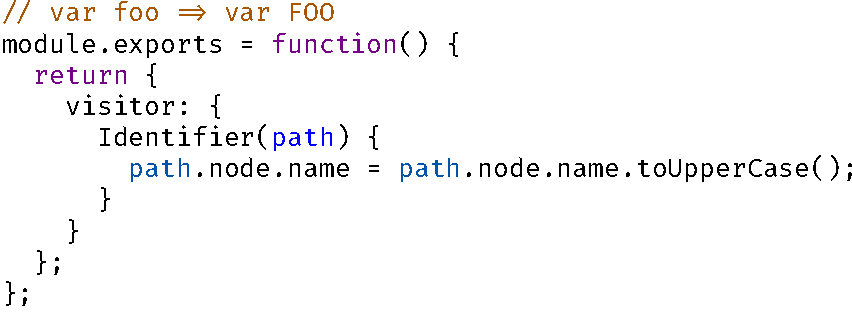
\includegraphics[width=0.6\textwidth]{src/2_Grundlagen/fig/minimal-babel-plugin.pdf}
  \caption[Minimalbeispiel eines Babel-Plugins]{Minimalbeispiel eines Babel-Plugins: Die Namen aller Bezeichner (\textit{Identifier}) werden in Großbuchstaben umgewandelt.}
  \label{code:babel-plugin-definition}
\end{figure}

% TODO: Was sind Pfade?

Im weiteren Verlauf wird sich die Untersuchung auf die zweite Phase, also der Transformation des abstrakten Syntaxbaums, konzentrieren, da hier die Lösung der vorliegenden Problemstellung realisiert wird. Das Parsen des Eingabquelltexts und das Generieren der Ausgabe kann durch Verwendung der gegebenen Bibliotheks-Funktionen von Babel simpel umgesetzt werden und bedarf keiner tiefgründigen Betrachtung.
